\documentclass[12pt,american]{article}

\usepackage[letterpaper,margin=1in]{geometry}
\pagestyle{plain}
\usepackage[T1]{fontenc}
\usepackage[utf8]{inputenc}
\usepackage[american]{babel}
\usepackage{csquotes}
\usepackage{lmodern}
\usepackage{setspace}
\usepackage[page,header]{appendix}
\usepackage{amsmath,amssymb}
\usepackage{booktabs}
\usepackage{array}
\usepackage{tabularx}
\usepackage{threeparttable}
\usepackage{longtable}
\usepackage{enumitem}
\usepackage{float}
\usepackage{graphicx}
\usepackage{caption}
\usepackage{subcaption}
\usepackage{xcolor}
\usepackage{tikz}
\usetikzlibrary{positioning,arrows.meta,calc}
\usepackage[round,sort]{natbib}
\usepackage[colorlinks=true,citecolor=blue,urlcolor=blue,linkcolor=black]{hyperref}
\usepackage{etoolbox}
\usepackage{footmisc}
\usepackage{datetime}

% Make only the year blue and hyperlinked in natbib author-year citations.
\makeatletter
\patchcmd{\NAT@citex}
  {\@citea\NAT@hyper@{%
     \NAT@nmfmt{\NAT@nm}%
     \hyper@natlinkbreak{\NAT@aysep\NAT@spacechar}{\@citeb\@extra@b@citeb}%
     \NAT@date}}
  {\@citea\NAT@nmfmt{\NAT@nm}%
   \NAT@aysep\NAT@spacechar\NAT@hyper@{\NAT@date}}{}{}
\patchcmd{\NAT@citex}
  {\@citea\NAT@hyper@{%
     \NAT@nmfmt{\NAT@nm}%
     \hyper@natlinkbreak{\NAT@spacechar\NAT@@open\if*#1*\else#1\NAT@spacechar\fi}{\@citeb\@extra@b@citeb}%
     \NAT@date}}
  {\@citea\NAT@nmfmt{\NAT@nm}%
   \NAT@spacechar\NAT@@open\if*#1*\else#1\NAT@spacechar\fi\NAT@hyper@{\NAT@date}}{}{}
\makeatother

\setcitestyle{round}
\renewcommand{\footnotelayout}{\doublespacing}
\newdateformat{monthyear}{\monthname[\THEMONTH] \THEYEAR}
\newcolumntype{L}[1]{>{\raggedright\arraybackslash}p{#1}}

\title{\textbf{Breaking the Great Firewall:}\\
\large A Field Experiment on Framed Foreign-News Exposure in China}
\author{Ziwen Zu\thanks{Department of Political Science, University of California, San Diego. Email: \href{mailto:zzu@ucsd.edu}{zzu@ucsd.edu}.}}
\date{\monthyear\today}

\begin{document}
\hypersetup{pageanchor=false}
\maketitle
\thispagestyle{empty}

\begin{abstract}
\noindent How does exposure to foreign media influence public opinion under authoritarian censorship? I address this question with a 12-week field experiment embedded in a major Chinese English test-preparation platform. The study randomized 6,365 participants (from a baseline pool of 12,215) into six arms varying article valence (pro-China vs.\ anti-China vs.\ neutral) and political dose (low vs.\ high), with an endline survey (\(N=5{,}215\)) and a follow-up survey (\(N=2{,}115\)). Three substantive findings stand out. First, foreign media effects are strongly valence-dependent: pro-China framing from Western outlets increases both regime support and trust in foreign media, while anti-China framing reduces regime support but simultaneously triggers nationalist backlash and source distrust — a mixed rather than uniformly liberalizing effect. Second, pro-China effects on regime support persist to the follow-up (marginal), whereas anti-China effects essentially vanish — asymmetric persistence consistent with a differential international legitimation mechanism. Third, weekly behavioral data and post-treatment willingness-to-pay reveal a complete mechanism chain: political content increases engagement equally across valences, but only pro-China content raises subsequent credibility ratings and demand for foreign news, while anti-China content suppresses demand — selective acceptance rather than selective avoidance. Together the results support a central claim: in authoritarian information environments, the political consequences of foreign media are determined not by source identity alone, but jointly by content valence, exposure dose, and the compatibility of message and audience prior beliefs.
\end{abstract}

\textbf{Keywords}: Authoritarianism; Censorship; China; Media; Public opinion

\newpage
\setcounter{page}{1}
\renewcommand{\thepage}{\arabic{page}}
\hypersetup{pageanchor=true}
\doublespacing

\section{Introduction}

Information control is a central instrument of authoritarian rule. In China, the state blocks major Western news websites through the Great Firewall while continuing to channel attention toward regime-compatible narratives \citep{kingpanroberts2013,roberts2018}. Yet censorship does not fully eliminate foreign information. English-learning platforms, study-abroad preparation, and digitally mediated educational content create indirect pathways through which Chinese citizens encounter foreign reporting in politically consequential ways. The empirical question is therefore not simply whether citizens can reach outside information, but what kinds of outside narratives they see, how often they see them, and whether they continue to seek them out after initial exposure.

Existing evidence points in different directions. Temporary access to blocked websites can reduce trust in the regime and expand political knowledge \citep{chenyang2019}. At the same time, foreign information can also improve evaluations of domestic governance when it corrects idealized views of the outside world \citep{huang2015international}. Foreign media effects in China are further filtered by selective exposure and prior beliefs about source credibility \citep{huangyeh2017,wangwestwood2024}. These mixed findings suggest that ``foreign media'' is too crude a treatment category. The effects of foreign information likely depend on framing, repetition, and the audience's willingness to accept the source as legitimate.

I address these issues with a randomized field experiment delivered through a large Chinese English test-preparation app. Over twelve weeks, participants receive two English-language readings per week, paired with close-reading videos, quizzes, and article ratings. The key manipulations are valence (pro-China versus anti-China), dose (low versus high), and benchmark content (apolitical China-related material and non-China neutral material). Because the app records article openings, watch time, quiz performance, and weekly interest and credibility ratings, the study does not rely on assignment alone. It directly observes whether participants consume, accept, and continue demanding politically charged foreign content.

The study contributes to research on authoritarian information control, persuasion, and selective exposure in four ways. First, it moves beyond simple ``access versus no access'' designs by isolating message valence and dose inside a common delivery environment. Second, it embeds the intervention in a repeated learning setting rather than a one-shot vignette, which makes habituation, backlash, and fatigue observable. Third, it combines attitudinal outcomes with behavioral measures of compliance and demand, making it possible to distinguish persuasion from avoidance. Fourth, it provides a transparent account of the realized study pipeline from recruitment to follow-up, which matters for evaluating inference in a politically sensitive online field experiment.

\section{Significance}

This project speaks directly to a core debate in comparative politics: whether information-based authoritarian control depends mainly on preventing access to foreign narratives, or whether authoritarian publics remain resilient even after repeated exposure to outside information \citep{gurievtreisman2019,stockmann2013,roberts2018}. If foreign criticism reliably lowers regime support, the findings suggest that censorship remains politically valuable because it suppresses politically costly comparisons. If, instead, foreign criticism generates backlash among nationalists or if pro-China stories from Western outlets improve evaluations of foreign media, then the political effects of uncensored information are more conditional than much of the democracy-promotion literature assumes.

The project also contributes to political communication research. Most work on selective exposure examines democratic contexts in which ideological media choice is abundant. China offers a different setting: citizens face a highly restricted information environment, yet they still sort among available cues and differ sharply in how they interpret outside information \citep{wangwestwood2024}. The app-based design shows how motivated reasoning, source credibility, and repeated exposure operate when access itself is politically structured.

Finally, the study contributes methodologically. Implementing a multi-month randomized field experiment on politically sensitive content inside China is unusual. The design pairs survey batteries with app-level measures of reading, viewing, and continued demand. That combination makes it possible to evaluate not only whether political attitudes shift, but also whether participants avoid, accept, or seek out more of the same information after treatment.

\section{Theory and Hypotheses}

\subsection{Theory}

Existing evidence suggests that Chinese public opinion is polarized between more nationalist, regime-supportive respondents and more liberal, regime-skeptical respondents. My argument centers on how foreign news interacts with those prior dispositions. Whether foreign news persuades, polarizes, or is simply ignored depends on four linked mechanisms: congruence with prior beliefs, source credibility, comparative benchmarking, and repeated exposure.

\textbf{Cognitive dissonance and congruence.} Respondents are more likely to accept information that fits their prior attitudes and more likely to resist or counter-argue information that sharply contradicts them \citep{taberlodge2006}. In this setting, anti-China coverage is more congruent for respondents who already distrust the regime, while pro-China coverage is more congruent for respondents with stronger nationalist priors. Congruent messages reinforce existing attitudes. Dissonant messages can fail to persuade or even produce backlash.

\textbf{Persuasion of the middle.} The strongest directional persuasion should appear among respondents who do not enter the study with strongly crystallized views. For this middle group, repeated exposure to foreign coverage can provide new comparative benchmarks without immediately triggering defensive rejection. In contrast, respondents at ideological extremes are more likely to process the same material through identity-protective reasoning.

\textbf{Information, identity, and out-group perceptions.} Foreign coverage does not only provide facts. It also signals how outside observers view China. Anti-China stories can therefore be interpreted either as credible external criticism or as hostile attacks from an out-group. Pro-China stories can either validate domestic pride or increase trust in Western outlets by revealing that they are not uniformly anti-China. These responses can reshape not only regime support but also media trust and broader affective attitudes toward foreign countries.

\textbf{Dose and habituation.} Repetition is theoretically ambiguous. Higher dose can strengthen learning and make a frame more cognitively accessible. But repeated exposure can also intensify reactance, lead to saturation, or suppress future demand for more of the same content. Dose is therefore not a mere implementation detail. It is a central part of the theory.

\textbf{Source credibility and prior foreign exposure.} Foreign information cannot persuade if it is discounted at the source stage \citep{hovlandweiss1951}. Participants who already consume foreign media, have studied abroad, or use workarounds to access blocked platforms should be more likely to treat Western outlets as credible. Respondents with low prior exposure may instead experience surprise, skepticism, or defensive rejection. I therefore expect prior foreign exposure and article-level credibility ratings to moderate treatment effects.

\subsection{Conceptual Framework}

The framework combines the receive-accept-sample logic of opinion formation \citep{zaller1992} with a simple Bayesian persuasion intuition \citep{kamenica2011bayesian}. Let \(R_{it}\in\{0,1\}\) indicate whether respondent \(i\) actually opens and consumes the assigned content in week \(t\). Conditional on reception, the probability of acceptance is
\[
\lambda_{it}
=
\omega_i \left[1-\rho\lvert S_f-I_{i0}\rvert\right],
\]
where \(\omega_i\) captures perceived source credibility, \(S_f\) indexes message valence, and \(I_{i0}\) captures baseline ideology. Congruent messages and more credible sources produce higher acceptance.

Accepted messages then accumulate as weighted signals:
\[
w_i(T)=\tau_0+\tau_s\sum_{t=1}^{T}R_{it}\lambda_{it},
\]
so the endline posterior for an outcome such as regime legitimacy becomes
\[
b_{i1}
=
\frac{\tau_0}{w_i(T)}b_{i0}
+
\frac{\tau_s}{w_i(T)}\sum_{t=1}^{T}R_{it}\lambda_{it}s_{it}.
\]
These expressions imply three empirical points. First, assignment and realized exposure are distinct. Second, dose matters because it changes the opportunity to receive and accept repeated signals. Third, heterogeneous treatment effects are not peripheral complications; they are part of the main theory.

\subsection{Hypotheses}

\begin{enumerate}[label=\textbf{H\arabic*.}, leftmargin=1.5em]
\item \textbf{Anti-China framing lowers regime support on average.} Relative to the non-China control arm, anti-China exposure decreases regime support, weakens support for censorship, and narrows the China--West feeling thermometer gap.
\item \textbf{Pro-China framing increases regime support on average.} Relative to the non-China control arm, pro-China exposure increases regime support and defensive nationalism, but may also increase trust in Western media by signaling that these outlets are not uniformly hostile.
\item \textbf{Apolitical China content differs from non-China neutral content.} Even without overt political valence, China-focused foreign content changes salience and can shift attitudes relative to non-China neutral material.
\item \textbf{High dose amplifies directional effects and backlash.} Within both the pro-China and anti-China arms, the high-dose condition produces larger absolute treatment effects than the low-dose condition.
\item \textbf{Baseline nationalism conditions persuasion.} Respondents with stronger baseline nationalism are more likely to reject anti-China content and more likely to respond favorably to pro-China content.
\item \textbf{Prior foreign exposure and credibility increase acceptance.} Treatment effects are larger among respondents with greater baseline foreign-media exposure and higher article-level credibility ratings.
\item \textbf{Dissonant high-dose exposure suppresses continued demand.} High-dose exposure to ideologically dissonant content reduces willingness to continue consuming similar foreign news, reflected in lower article-liking scores, lower willingness to pay, and lower follow-up signup.
\end{enumerate}

\section{Research Design}

\subsection{Context, Sample, and Recruitment}

I ran the experiment in partnership with a major Chinese test-preparation company whose mobile app supports recorded videos, quizzes, article delivery, and backend learning analytics. The study population consists of young adult users preparing for TOEFL, IELTS, GRE, GMAT, and related English examinations. This population is analytically useful because participants regularly consume English materials while remaining embedded in a censored domestic information environment.

Recruitment occurred through in-app invitations encouraging users to join a training camp for intensive study of authentic English materials. Participation was voluntary and did not affect grades or access to ordinary coursework. The recruitment pipeline generated 59,901 clicks in May 2025, 22,317 survey starts, and 12,215 participants who passed the prescreen, provided contact information, and completed the baseline survey in June 2025. Among those respondents, 6,365 were block-randomized and contacted for consent confirmation and verification of content-delivery methods.

The baseline survey served two purposes. First, it collected the blocking variables used in randomization: gender, region, English proficiency, and baseline nationalism. Second, it gathered pre-treatment measures of ideology, media trust, censorship attitudes, and foreign exposure. To reduce sensitivity, ideological items appeared inside a broader client-profile module, while foreign-media exposure items appeared inside a market-research module about study-abroad interests and international media habits. Direct questions about VPN use were avoided; instead, the survey asked whether respondents accessed platforms and outlets that typically require circumvention inside China.

\subsection{Sample Size, Realized Flow, and Power}

The participant flow in Figure~\ref{fig:flow} is the authoritative sample record for the study. The randomized sample is \(N=6{,}365\), the weekly-and-endline sample is \(N=5{,}215\), and the follow-up sample is \(N=2{,}115\). Under near-equal allocation across six arms, this implies approximately \(n=1{,}061\) participants per arm at randomization, \(n=869\) per arm at endline, and \(n=353\) per arm at follow-up.

Power calculations use standardized outcomes (\(\sigma=1\)), two-sided tests, 80 percent power, and \(R^2=0.30\) for ANCOVA specifications with baseline outcomes and block fixed effects:
\[
\text{MDE}=
\left(z_{1-\alpha/2}+z_{0.80}\right)
\sqrt{\frac{2(1-R^2)}{n}}.
\]

\begin{table}[H]
\centering
\caption{Power Benchmarks Using the Realized Flow Counts}
\label{tab:power_mde}
\footnotesize
\begin{tabularx}{\textwidth}{@{}L{0.41\textwidth}L{0.22\textwidth}L{0.17\textwidth}L{0.17\textwidth}@{}}
\toprule
Estimand family & Effective comparison size & Randomized sample MDE & Endline sample MDE \\
\midrule
Pairwise arm contrast (for example, Anti-high vs Non-China), nominal \(\alpha=0.05\) & \(1061\) vs \(1061\) or \(869\) vs \(869\) & 0.102 & 0.112 \\
Pairwise arm contrast, Holm benchmark \(\alpha=0.0167\) & \(1061\) vs \(1061\) or \(869\) vs \(869\) & 0.118 & 0.130 \\
Pooled political exposure (four arms) vs Non-China control, nominal \(\alpha=0.05\) & \(4244\) vs \(1061\) or \(3476\) vs \(869\) & 0.080 & 0.089 \\
Pooled political exposure (four arms) vs Non-China control, Holm benchmark \(\alpha=0.0167\) & \(4244\) vs \(1061\) or \(3476\) vs \(869\) & 0.093 & 0.103 \\
Within-valence dose contrast (High vs Low), nominal \(\alpha=0.05\) & \(1061\) vs \(1061\) or \(869\) vs \(869\) & 0.102 & 0.112 \\
\bottomrule
\end{tabularx}
\end{table}

The follow-up sample is much smaller, so pairwise MDEs rise to approximately 0.176 SD under nominal thresholds and 0.204 SD under Holm-adjusted thresholds. I therefore treat follow-up estimates as substantively important but less precisely estimated than endline results.

\subsection{Experimental Treatment Conditions}

The implemented design follows a six-arm structure. Participants were assigned to one of four political treatment cells from a Pro-China/Anti-China by High/Low dose design, or to one of two benchmark arms: apolitical China-related content or non-China neutral content. Every participant received 24 content slots over 12 weeks.

\begin{table}[H]
\centering
\caption{Treatment Arms and Content Schedule}
\label{tab:arms}
\begin{threeparttable}
\small
\begin{tabularx}{\textwidth}{L{0.25\textwidth}L{0.18\textwidth}L{0.15\textwidth}X}
\toprule
Arm & Political dose & Total readings & Content description \\
\midrule
Pro-China, low dose & 6 political pieces & 24 & 6 pro-China political pieces plus 18 neutral fillers. \\
Pro-China, high dose & 24 political pieces & 24 & 24 pro-China political pieces across the full intervention. \\
Anti-China, low dose & 6 political pieces & 24 & 6 anti-China political pieces plus 18 neutral fillers. \\
Anti-China, high dose & 24 political pieces & 24 & 24 anti-China political pieces across the full intervention. \\
Apolitical China & 12 apolitical-China items & 24 & China-related but non-political content plus 12 neutral fillers. \\
Non-China control & 0 China-political pieces & 24 & Neutral non-China content matched on difficulty and workload. \\
\bottomrule
\end{tabularx}
\begin{tablenotes}
\footnotesize
\item All arms received two readings per week, paired with instructional videos, quizzes, and article ratings.
\end{tablenotes}
\end{threeparttable}
\end{table}

\subsection{Content Preparation, Delivery, and Compliance}

The final materials bank contains 89 unique readings: 24 pro-China political pieces, 24 anti-China political pieces, 17 apolitical China-related pieces, and 24 non-China controls. Unlike earlier drafts, the realized bank is source-diversified rather than concentrated in only a few elite newspapers. The overtly political pools draw mainly from \emph{Reuters}, \emph{AP News}, \emph{The Guardian}, \emph{The Economist}, \emph{The Washington Post}, and \emph{The New York Times}. By contrast, the benchmark pools rely more heavily on \emph{Smithsonian}, \emph{National Geographic}, \emph{The Guardian}, and a smaller number of \emph{Washington Post} and \emph{CNN Travel} pieces. This diversification reduces the risk that respondents simply react to a single outlet label instead of to the substantive content of the reading, while also avoiding a benchmark pool made up only of city-guide or service-journalism copy.

The pro-China pool emphasizes favorable coverage of economic management, green development, industrial upgrading, technological capacity, and policy support. The anti-China pool emphasizes censorship, surveillance, social strain, property-market distress, financial fragility, and governance failures. The apolitical-China pool focuses on food, travel, urban culture, history, arts, and society. The non-China control pool is likewise heterogeneous: rather than relying only on city-guide pieces, it mixes travel, museums, culture, food, and place-based features unrelated to China. All selected readings predate the June 2025 intervention launch.

To reduce unnecessary political sensitivity, the content excludes highly taboo subjects such as Tiananmen, Xinjiang, religion, ethnic conflict, and direct personal criticism of top leaders. The focus is on policy performance, international evaluation, and soft power rather than on core political red lines. Before classroom use, each source article was converted into a clean plain-text reading version with navigation menus, promotional modules, links, image captions, and other web artifacts removed. Texts were then screened for classroom suitability and embedded in a common app format, paired with a professionally recorded close-reading video explaining vocabulary, grammar, and translation issues. Presentation was standardized across arms so that differences in response reflect message content rather than differences in pedagogical support.

As a post-curation content-validity check, I score the finalized plain-text corpus using an article-level China-valence measure. This exercise is conceptually similar to press-level validity checks in related work on Western coverage of China, such as the evidence in Chen and Han's \emph{Economic Journal} study showing systematically more negative English-language Western coverage than \emph{China Daily} on an embedding-based scale. My teaching version uses a simpler domain-specific measure: it scores only China-anchored sentences and contrasts pro-China policy terms with anti-China criticism terms, with criticism terms receiving a modestly heavier weight so that anti-China framing is not diluted by neutral macro-policy nouns. In the finalized teaching bank, the directional contrast in the political pools is now clear and roughly symmetric: pro-China articles average \(+0.490\), while anti-China articles average \(-0.432\). At the same time, the benchmark pools remain close to neutrality: the apolitical-China pool averages \(-0.063\), and the non-China control pool averages \(-0.019\), with both confidence intervals spanning zero. I therefore use the content-validity diagnostics primarily to verify the intended pro-versus-anti polarity of the political pools while keeping the benchmark pools near a substantively neutral baseline. Topic-level diagnostics reinforce this interpretation: anti-China policy and social-stress pieces are the most negative subgroup (\(-0.961\) on average), anti-China censorship and repression pieces are also strongly negative (\(-0.809\)), and the non-China benchmark subgroups closest to neutral are travel/place and ``other'' pieces (\(0.000\) on average).

As a separate non-substantive comparability check, I also measured article-level word count, average sentence length, average word length, and Flesch--Kincaid grade. After applying a common \(950\) to \(1{,}050\)-word excerpt window to longer benchmark texts, article length is far more comparable across banks: the mean cleaned article now contains about \(722\) words in the pro-China pool, \(898\) in the anti-China pool, \(846\) in the apolitical-China pool, and \(987\) in the non-China control pool. Sentence length and general readability are now also closely aligned across banks. The omnibus \(p\)-values are \(0.90\) for average sentence length and \(0.93\) for Flesch--Kincaid grade; the corresponding \(p\)-value for word count falls to \(0.001\), indicating that remaining differences are much smaller than in the untrimmed corpus. Simulated assignment-level diagnostics show the same convergence at the realized bundle level: on slot-1 exposure, average article length ranges from roughly \(723\) words in the pro-high arm to \(987\) in the control arm, with the apolitical-China arm at \(845\) and the anti-high arm at \(902\). I therefore treat textual balance as an explicit design diagnostic rather than an unexamined assumption, and I report these checks alongside the main content-validity evidence.

Every Monday the app unlocked two new readings and two corresponding videos. By the end of the week, participants completed the readings, watched the videos, answered a ten-item quiz, and rated each article on interest, credibility, and whether they wanted more similar content. A participant counted as compliant for a given week after meeting the watch-time threshold and reaching the quiz benchmark. These repeated measures make it possible to distinguish assigned treatment from realized exposure and acceptance.

\subsection{Block Randomization}

I implemented individual-level block randomization to improve balance across treatment arms. Blocks were constructed from gender, English proficiency, baseline nationalism, and region, yielding 24 strata. Within each stratum, the app backend shuffled user IDs and allocated participants as evenly as possible across the six arms. Small remainder differences arose mechanically from within-block integer allocation, but the final design remains close to equal assignment.

Because the same app handled consent confirmation, content delivery, and behavioral logging, randomization remained invisible to ordinary teaching staff and other users. After enrollment closed, I assessed covariate balance with stratum-adjusted tests and standardized mean differences.

\subsection{Outcome Measures and Questionnaire Modules}

The questionnaire architecture in this proposal follows the structure developed in the earlier \texttt{Censorship/Main} draft, but the wording and measurement schedule are aligned to the realized six-arm study. Self-report instruments appear at baseline, endline, and follow-up unless otherwise noted, while weekly in-app ratings capture immediate reactions to assigned content.

\begin{table}[H]
\centering
\caption{Questionnaire and Measurement Modules}
\label{tab:questionnaire}
\footnotesize
\begin{tabularx}{\textwidth}{@{}L{0.20\textwidth}L{0.18\textwidth}L{0.39\textwidth}L{0.17\textwidth}@{}}
\toprule
Module & Construct & Example content & Wave \\
\midrule
Client profile & Demographics, education, test preparation & Age, gender, province, exam type, recent English scores & Baseline \\
International outlook & Regime support, nationalism, China--West affect & Satisfaction with economic development and government efficiency; feelings toward China and Western democracies & Baseline, endline, follow-up \\
Media environment & Censorship attitudes, media trust, foreign exposure & Support for restricting online content; trust in domestic state, domestic commercial, and Western media; access to foreign platforms and outlets & Baseline, endline, follow-up \\
Weekly reaction module & Acceptance and demand & Article interest, perceived credibility, willingness to see similar stories, quiz accuracy, watch time & Weekly \\
Knowledge check & Factual learning & Multiple-choice questions tied to treatment content, plus placebo items & Endline, follow-up \\
Behavioral demand & Continued demand, spillovers, and post-study trajectories & WTP for continued access to foreign news, digest signup and use, discussion and sharing, selective avoidance, and English-study or application updates & Endline, follow-up \\
\bottomrule
\end{tabularx}
\end{table}

\paragraph{Primary attitudinal outcomes.}
The core outcome battery is adapted from the older Main draft and retains the same substantive constructs:
\begin{enumerate}[label=\arabic*., leftmargin=1.5em]
\item \textbf{Regime-support index.} A standardized index averaging satisfaction with economic development, social stability, social equality, technological progress, and government efficiency.
\item \textbf{Censorship-attitude scale.} Three items measuring endorsement of information control, including agreement that restricting some online content is necessary for social stability.
\item \textbf{China--West feeling thermometer gap.} Separate 0--100 ratings of China and Western democracies, differenced so that higher values indicate relatively warmer feelings toward China.
\item \textbf{Nationalism battery.} Four items capturing patriotic attachment and defensive nationalism, including agreement that foreign criticism of China is usually biased.
\end{enumerate}

\paragraph{Behavioral and secondary outcomes.}
The study also records willingness to pay for continued foreign-news access, article-level credibility and interest ratings, quiz performance, reading duration, video watch time, and follow-up signup for a foreign-news digest. To sharpen the mechanism tests, the endline and follow-up surveys additionally measure source-specific credibility, ideological congruence, emotional reactions, off-platform foreign-news consumption, discussion and sharing behavior, selective avoidance or self-censorship, and the perceived English-learning value of the materials. For this population of test-prep users, the follow-up survey also records exam-taking, score updates, and study-abroad application progress so that persistent treatment effects can be distinguished from later changes in educational incentives.

\paragraph{Instrument quality.}
Question wording follows the structure used in the older \texttt{Censorship/Main} questionnaire plan: politically sensitive items are embedded inside broader modules on international outlook, media habits, and study-abroad preparation. Item order is randomized within batteries, each survey contains attention checks, and the backend time-stamps all responses and behavioral logs. Because all data are collected inside the app, survey records, quiz scores, and engagement metrics can be linked through the study ID without exposing personally identifying information to the research team.

\subsection{Attrition and Mitigation Strategy}

Attrition is non-trivial in a 12-week online field experiment. The realized participant flow makes that clear: 6,365 randomized participants, 5,215 endline respondents, and 2,115 follow-up respondents. The study used weekly reminders, low-friction participation rules, and completion incentives to reduce dropout. Participants who completed the program received premium course benefits inside the app, and weekly quiz performance triggered small additional vouchers. Incentives depended on participation and quiz completion rather than on political responses.

In analysis, I keep intention-to-treat estimates as the primary estimand. Attrition adjustments include inverse-probability weighting, Lee bounds where differential attrition is relevant, and multiple imputation conditioned on baseline covariates and interim engagement metrics.

\begin{figure}[H]
\centering
\scalebox{0.7}{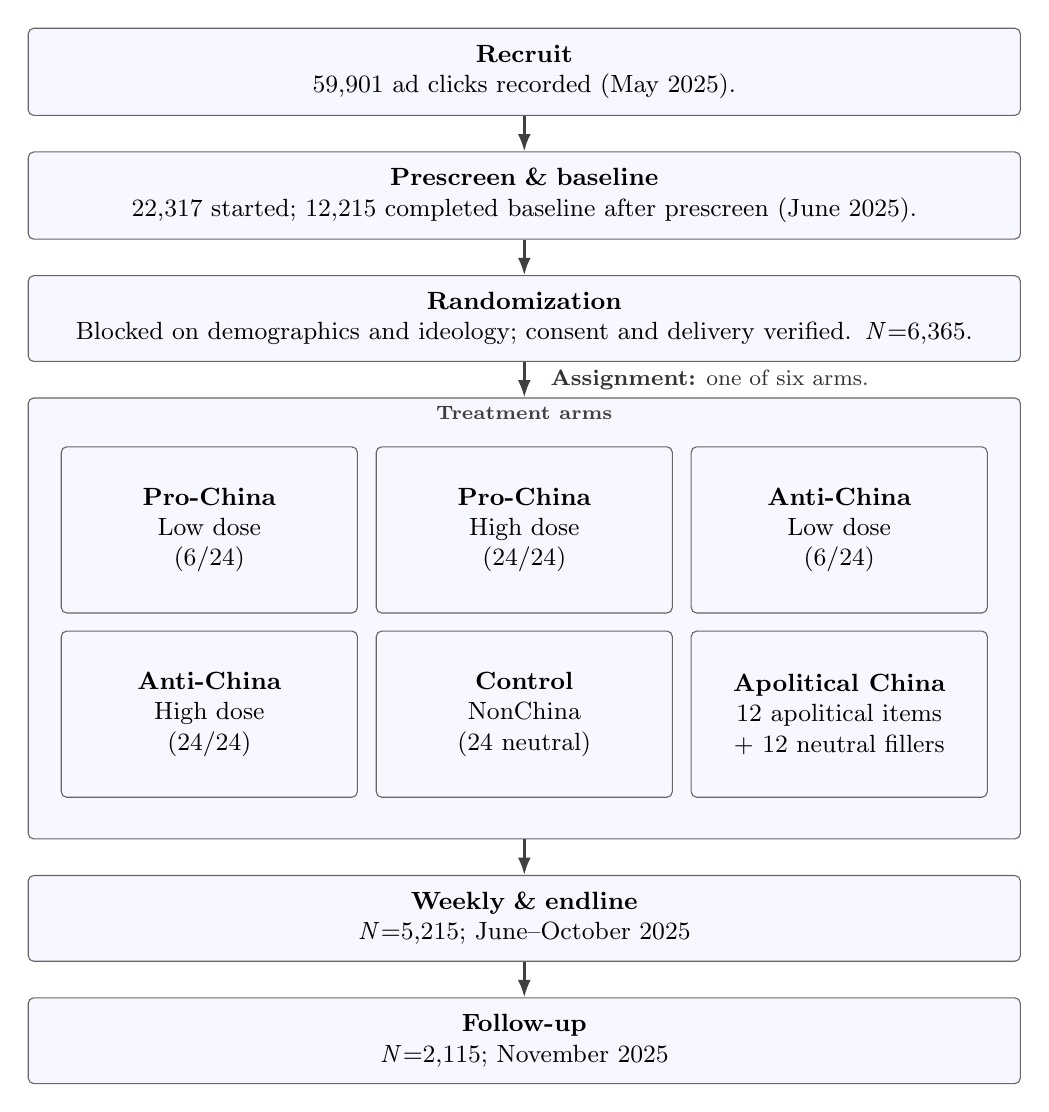
\begin{tikzpicture}[
  x=1cm, y=1cm,
  every node/.style={font=\small},
  % Outer width matches the six-arm container (group); text area = width minus inner sep
  main/.style={
    draw=black!60,
    fill=blue!3,
    rounded corners=2pt,
    align=center,
    minimum width=12.6cm,
    text width=\dimexpr12.6cm-12pt\relax,
    minimum height=1.0cm,
    inner sep=6pt
  },
  group/.style={
    draw=black!60,
    fill=blue!3,
    rounded corners=2pt,
    minimum width=12.6cm,
    minimum height=5.6cm,
    inner sep=0pt
  },
  arm/.style={
    draw=black!60,
    fill=blue!3,
    rounded corners=2pt,
    align=center,
    inner sep=3pt
  },
  arr/.style={-{Latex[length=2.2mm]}, line width=0.9pt, draw=black!75},
  arrlabel/.style={font=\footnotesize, text=black!80, align=left}
]

% Uniform vertical shaft length between stacked boxes (south of upper → north of lower)
\def\flowarrowgap{0.45}

\node[main] (recruit) at (0,0) {\textbf{Recruit}\\59,901 ad clicks recorded (May 2025).};

\node[main, anchor=north] (screen) at ($(recruit.south)+(0,-\flowarrowgap)$) {\textbf{Prescreen \& baseline}\\22,317 started; 12,215 completed baseline after prescreen (June 2025).};
\node[main, anchor=north] (rand) at ($(screen.south)+(0,-\flowarrowgap)$) {\textbf{Randomization}\\Blocked on demographics and ideology; consent and delivery verified. \textit{N}=6,365.};
\node[group, anchor=north] (armsbox) at ($(rand.south)+(0,-\flowarrowgap)$) {};

% Panel label: single line, tight to top border; arm cells start lower so nothing overlaps
\node[font=\scriptsize\bfseries, text=black!75, anchor=north, inner sep=0pt] at ($(armsbox.north)+(0,-0.10)$) {Treatment arms};

% Six equal cells (3x2) — row offsets leave ~0.45cm below the label for descenders / padding
\node[arm, anchor=north] (pl) at ($(armsbox.north)+(-4.00,-0.62)$) {\parbox[c][1.90cm][c]{3.55cm}{\centering\textbf{Pro-China}\\Low dose\\(6/24)}};
\node[arm, anchor=north] (ph) at ($(armsbox.north)+(0,-0.62)$) {\parbox[c][1.90cm][c]{3.55cm}{\centering\textbf{Pro-China}\\High dose\\(24/24)}};
\node[arm, anchor=north] (al) at ($(armsbox.north)+(4.00,-0.62)$) {\parbox[c][1.90cm][c]{3.55cm}{\centering\textbf{Anti-China}\\Low dose\\(6/24)}};
\node[arm, anchor=north] (ah) at ($(armsbox.north)+(-4.00,-2.96)$) {\parbox[c][1.90cm][c]{3.55cm}{\centering\textbf{Anti-China}\\High dose\\(24/24)}};
\node[arm, anchor=north] (nc) at ($(armsbox.north)+(0,-2.96)$) {\parbox[c][1.90cm][c]{3.55cm}{\centering\textbf{Control}\\NonChina\\(24 neutral)}};
\node[arm, anchor=north] (ac) at ($(armsbox.north)+(4.00,-2.96)$) {\parbox[c][1.90cm][c]{3.55cm}{\centering\textbf{Apolitical China}\\12 apolitical items\\+ 12 neutral fillers}};

\node[main, anchor=north] (endline) at ($(armsbox.south)+(0,-\flowarrowgap)$) {\textbf{Weekly \& endline}\\\textit{N}=5,215; June--October 2025};
\node[main, anchor=north] (follow) at ($(endline.south)+(0,-\flowarrowgap)$) {\textbf{Follow-up}\\\textit{N}=2,115; November 2025};

% Connectors: equal-length vertical segments
\draw[arr] (recruit.south) -- (screen.north);
\draw[arr] (screen.south) -- (rand.north);
\draw[arr] (rand.south) -- (armsbox.north)
  node[pos=0.5, anchor=west, xshift=2mm, arrlabel] {\textbf{Assignment:} one of six arms.};
\draw[arr] (armsbox.south) -- (endline.north);
\draw[arr] (endline.south) -- (follow.north);

\end{tikzpicture}
}
\caption{Implemented participant flow and study structure.}
\label{fig:flow}
\end{figure}

\section{Empirical Strategy}

\subsection{Main intention-to-treat estimates}

The primary analysis estimates intention-to-treat effects using ANCOVA models with block fixed effects:
\[
Y_{i1}
=
\alpha
+
\sum_{a=1}^{5}\beta_a\mathbf{1}\{A_i=a\}
+
\gamma Y_{i0}
+
\lambda_{b(i)}
+
X_i^\prime\delta
+
\varepsilon_i,
\]
where \(Y_{i1}\) is the endline outcome, \(Y_{i0}\) is the baseline value of the same outcome, \(A_i\) indexes assignment to one of the five non-reference treatment arms, and \(\lambda_{b(i)}\) are block fixed effects. The non-China control arm is the omitted reference category.

The most important confirmatory contrasts are:
\begin{enumerate}[label=\arabic*., leftmargin=1.5em]
\item pooled Anti-China treatments versus the non-China control arm;
\item pooled Pro-China treatments versus the non-China control arm;
\item apolitical China versus the non-China control arm;
\item high-versus-low dose contrasts within the pro-China and anti-China arms.
\end{enumerate}

\subsection{Heterogeneity, compliance, and dose response}

I estimate heterogeneous treatment effects by interacting assignment with baseline nationalism, baseline regime support, and prior foreign-media exposure. These moderators map directly onto the theoretical framework: ideological congruence, prior credibility, and selective reception.

Because the app records article openings, reading time, watch time, and quiz completion, I also distinguish assignment from realized exposure. I use randomized assignment as an instrument for realized political exposure to estimate complier-average effects and dose-response relationships. These models clarify whether small average effects arise because messages fail to persuade or because participants selectively avoid assigned content.

\subsection{Dynamic outcomes, attrition, and inference}

The panel structure of the data permits endline and follow-up analyses with participant-level fixed effects:
\[
Y_{it}
=
\mu_i
+
\lambda_t
+
\beta_1(T_i\times\mathbf{1}\{t=1\})
+
\beta_2(T_i\times\mathbf{1}\{t=2\})
+
\epsilon_{it},
\]
where \(t=0\) denotes baseline, \(t=1\) endline, and \(t=2\) follow-up. These specifications show whether treatment effects persist, decay, or reverse after the weekly intervention ends.

Inference uses heteroskedasticity-robust standard errors with block fixed effects for participant-level regressions and participant-clustered standard errors for weekly panel outcomes. I report randomization-inference \(p\)-values for the main confirmatory contrasts, bootstrap confidence intervals for nonlinear dose-response and dispersion estimands, and Holm-adjusted \(p\)-values for the primary outcome family. Secondary outcomes are reported with false-discovery-rate adjusted \(q\)-values \citep{haalandrothwohlfart2023}.

\section{Timeline and Feasibility}

The study timeline is anchored to the completed 2025 fieldwork rather than to earlier scheduling assumptions.

\begin{table}[H]
\centering
\caption{Field Timeline}
\label{tab:timeline}
\begin{tabularx}{\textwidth}{@{}L{0.34\textwidth}X@{}}
\toprule
Date & Activity \\
\midrule
May 2025 & Recruitment campaign generated 59,901 clicks through the app. \\
June 2025 & 22,317 respondents started the survey; 12,215 completed the prescreen and baseline survey. \\
Late June 2025 & 6,365 participants were block-randomized and contacted for consent and delivery verification. \\
June--October 2025 & Twelve-week intervention with weekly quizzes, article ratings, and app-level compliance logs. \\
June--October 2025 & Endline survey completed by 5,215 respondents. \\
November 2025 & Follow-up survey completed by 2,115 respondents. \\
\bottomrule
\end{tabularx}
\end{table}

Operationally, the study is feasible because it relies on an existing app infrastructure and never requires participants to install VPN software or directly visit blocked websites. Relative to the platform's user base, the realized randomized sample is modest: 6,365 randomized participants amount to only a small share of the broader app population. That scale helps explain why recruitment through a large educational platform is realistic even in a sensitive research environment.

\section{Deviations from the Registered PAP}

The implemented study differs from parts of the preregistered PAP and related metadata records. Two deviations matter most for interpretation.

First, the implemented design is the six-arm structure shown in Figure~\ref{fig:flow}: Pro-China/Anti-China crossed with High/Low dose, plus an apolitical-China benchmark arm and a non-China control arm. Some earlier study materials described additional arms or alternative treatment structures that were not carried into the final implementation. All analyses in this proposal use the implemented six-arm design.

Second, the sample-size fields across study documents are not fully consistent. In particular, some metadata records report a sample size of 6,000, whereas the realized participant flow shows 6,365 randomized participants, 5,215 endline respondents, and 2,115 follow-up respondents. In this proposal, the realized flow chart is the authoritative source. All descriptive statistics, power calculations, estimands, and inferential statements are keyed to those final counts.

These deviations do not require abandoning the PAP's theoretical core. The central hypothesis families remain intact: foreign political framing, exposure dose, source credibility, and selective engagement. What changes is the operational mapping from those hypothesis families to the implemented six-arm design and the realized sample sizes.

\section{Ethical Considerations}

This project received Institutional Review Board approval at UC San Diego on May 28, 2025. The core ethical challenge is not ordinary survey burden, but the combination of politically sensitive content, repeated exposure, and high-frequency behavioral logging inside China. I therefore adapt the ethics language from the older \texttt{Censorship/RR} draft to the realized study.

\subsection{Informed Consent and Participant Autonomy}

Participants completed informed consent in Chinese before enrollment. The consent language explained that the study involved reading English materials, watching videos, taking quizzes, and answering surveys about media and social issues. The form emphasized voluntariness, the right to skip any question, and the right to stop participating without losing already earned compensation.

To reduce anxiety without misleading respondents, the consent form did not foreground words such as ``censorship'' or ``political attitudes.'' Instead, it described the project in terms of English learning and media exposure while still making clear that some articles concerned governments, current events, and international evaluations.

\subsection{Risk, Privacy, and Data Security}

\textbf{Psychological risk.} The most immediate participant burden is mild discomfort from reading ideologically dissonant material. To reduce that burden, the content pool excluded highly taboo or graphic topics, participants could skip questions at any point, and withdrawal did not require justification. This design keeps the study within a minimal-risk profile while still allowing exposure to politically meaningful foreign content.

\textbf{Political and social risk.} A more sensitive concern is whether participants might worry that their assignment or responses could become visible to others. The study addresses that risk by keeping all delivery inside a password-protected educational app. Instructors and classmates did not observe individual assignment, completion patterns, or survey responses, and the research team received de-identified records only.

\textbf{Legal and regulatory risk.} The intervention exposed respondents to foreign political content in a censored media environment, so the content itself was curated conservatively. The study relied on ordinary educational delivery channels already present in the partner app, and the article set avoided especially sensitive topics and direct criticism of top leaders. Source articles were prepared from lawfully accessed originals, including public webpages, subscription access, and ordinary instructional preparation by the partner company. Because many of those originals remain copyrighted, any public replication archive will report bibliographic metadata, URLs, coding decisions, and derived measures rather than redistribute publisher full text. These choices reduced foreseeable legal and administrative risk without altering the study's core comparison between positive, negative, apolitical, and neutral foreign content.

\textbf{Data-security risk.} The most credible harm channel in this project is data linkage. The data architecture therefore separates identities from research records. Personally identifying information remained on company servers, while the research team worked with de-identified data keyed to study IDs. The link file used for compensation was retained only as long as operationally necessary and then destroyed. Public-facing materials report aggregate outcomes or disclosure-screened extracts rather than raw behavioral traces.

\subsection{Debriefing and Post-Study Rights}

Participants received debriefing information at the end of the study and again at follow-up. The debrief explained the purpose of varying article framing and dose and reminded respondents of their right to request deletion of identifiable records before final de-identification. Control-group access to additional foreign-news materials after the study reduced inequity in exposure.

\section{Conclusion}

This proposal analyzes a completed field experiment on foreign-news exposure in China. The study combines a large realized randomized sample, repeated exposure, behavioral compliance logs, and multiple survey waves. Its main value is not only in estimating whether pro-China or anti-China content shifts regime support, but also in showing when foreign information persuades, when it backfires, and when it suppresses its own future demand. By aligning theory, design, inference, and ethics to the final participant flow, the proposal presents the study on its actual empirical terms rather than on the shifting sample-size placeholders that appeared in earlier drafts and metadata records.

\newpage
\hypersetup{pageanchor=false}
\appendix
\section*{Supplementary Material}
\setcounter{page}{0}
\thispagestyle{empty}
\newpage
\renewcommand{\thepage}{SI-\arabic{page}}
\hypersetup{pageanchor=true}
\setcounter{figure}{0}
\renewcommand{\thefigure}{SI.\arabic{figure}}
\setcounter{table}{0}
\renewcommand{\thetable}{SI.\arabic{table}}

\section{Questionnaire}

This appendix records the questionnaire structure used in the study. The full instrument was administered in Chinese inside the partner app, with English source wording retained for archival and coding purposes. Politically sensitive items were embedded inside broader modules on study-abroad preparation, media habits, and international outlook.

\subsection*{Appendix Contents}
\begin{itemize}
\item \hyperref[app:background]{Background and Demographics}
\item \hyperref[app:media]{Media Exposure and Foreign Orientation}
\item \hyperref[app:attitudes]{Primary Attitude Batteries}
\item \hyperref[app:knowledge]{Issue-Specific and Knowledge Items}
\item \hyperref[app:weekly]{Weekly In-App Module}
\item \hyperref[app:endline]{Endline and Follow-Up Behavioral Measures}
\item \hyperref[app:qc]{Survey Quality Controls}
\item \hyperref[app:refs]{References}
\end{itemize}

\subsection{Background and Demographics}\label{app:background}

\begin{enumerate}[label=\arabic*., leftmargin=1.5em]
\item Gender.
\item Age range.
\item Ethnicity.
\item Highest educational attainment.
\item Current city of residence.
\item Political affiliation or party identification.
\item Examination currently being prepared for (TOEFL, IELTS, GRE, GMAT, or other).
\item Most recent score on that examination.
\item Length of time spent preparing for the examination.
\item Main motivation for joining the foreign-news study program.
\end{enumerate}

\subsection{Media Exposure and Foreign Orientation}\label{app:media}

\begin{enumerate}[label=\arabic*., leftmargin=1.5em]
\item \textbf{News-consumption frequency.} ``In the past 90 days, how often have you consumed news from the following sources?'' Response scale: 1 = Never, 5 = Very often.
\begin{itemize}
\item Chinese state-run news websites.
\item Chinese commercial news apps.
\item Social media platforms.
\item Foreign news websites in English.
\item Foreign-language YouTube news channels.
\item News shared by friends or family through chat groups.
\end{itemize}
\item \textbf{Media-trust battery.} ``How much do you trust content from the following media platforms?'' Separate items for state media, commercial Chinese media, social media, foreign English-language outlets, foreign YouTube channels, and chat-group news sharing.
\item Frequency of reading foreign news by any means during the previous month.
\item Whether the respondent has an account on or has visited TikTok, Facebook, Twitter, YouTube, or Instagram.
\item Whether the respondent has ever traveled or lived outside Mainland China.
\item Whether the respondent plans to study or live abroad within the next few years.
\end{enumerate}

\subsection{Primary Attitude Batteries}\label{app:attitudes}

\begin{enumerate}[label=\arabic*., leftmargin=1.5em]
\item \textbf{Regime-support index.} ``How satisfied are you with the current situation in China in the following areas?'' Response scale: 1 = Very satisfied, 5 = Very unsatisfied.
\begin{itemize}
\item Economic development.
\item Social stability.
\item Social equality.
\item Technological progress.
\item Government efficiency.
\end{itemize}
\item \textbf{Censorship-attitude scale.} ``Please indicate your level of agreement with the following statements about censorship and content regulation.'' Response scale: 1 = Strongly disagree, 5 = Strongly agree.
\begin{itemize}
\item Restricting certain online content is necessary for social stability.
\item The government has the right to censor politically sensitive news.
\item Citizens should be protected from information that may cause political disorder.
\end{itemize}
\item \textbf{China--West feeling thermometers.} ``Please rate your feelings toward China'' and ``Please rate your feelings toward Western democracies'' on separate 0--100 scales.
\item \textbf{Nationalism battery.} Response scale: 1 = Strongly disagree, 5 = Strongly agree.
\begin{itemize}
\item Foreign criticism of China is usually biased.
\item China should resist outside pressure even when foreign countries object.
\item I feel proud when I see China praised internationally.
\item Western countries often judge China unfairly.
\end{itemize}
\end{enumerate}

\subsection{Issue-Specific and Knowledge Items}\label{app:knowledge}

\begin{enumerate}[label=\arabic*., leftmargin=1.5em]
\item Policy items tied to the main content banks: economics, domestic development, culture and society, and science and technology.
\item Factual multiple-choice questions about claims appearing in treatment articles.
\item Placebo knowledge items on topics not covered in the weekly materials.
\end{enumerate}

\subsection{Weekly In-App Module}\label{app:weekly}

Each week participants completed the following module for the assigned readings:

\begin{enumerate}[label=\arabic*., leftmargin=1.5em]
\item Article open and reading log.
\item Video watch-time log.
\item Ten-item comprehension quiz.
\item ``How interesting did you find this article?'' Response scale: 0--100.
\item ``How credible did you find this article?'' Response scale: 0--100.
\item ``Would you like to read similar content in the future?'' Response scale: 0--100.
\end{enumerate}

\subsection{Endline and Follow-Up Behavioral Measures}\label{app:endline}

\begin{enumerate}[label=\arabic*., leftmargin=1.5em]
\item \textbf{Endline core outcomes.} Repeat administration of the core media-trust, regime-support, censorship, nationalism, and China--West affect batteries immediately after the intervention.
\item \textbf{Source credibility and interpretive reactions.} ``Thinking about the foreign outlets used in this program, how much do you agree with the following statements?'' Response scale: 1 = Strongly disagree, 5 = Strongly agree.
\begin{itemize}
\item The foreign outlets in this program usually provided useful information about China.
\item The foreign outlets in this program were fair in how they described China.
\item The foreign outlets in this program were biased against China.
\item The foreign outlets in this program helped me understand Chinese society better.
\item Many of the articles felt close to my own views.
\end{itemize}
\item \textbf{Psychological reactions to the treatment.} ``Across the study as a whole, how often did the assigned materials make you feel the following?'' Response scale: 1 = Never, 5 = Very often.
\begin{itemize}
\item Curious.
\item Proud.
\item Angry or defensive.
\item Embarrassed or uncomfortable.
\item More confident in my own political views.
\item More uncertain about my previous views.
\end{itemize}
\item \textbf{Behavioral demand for future foreign news.}
\begin{itemize}
\item Maximum amount the respondent was willing to give up from the participation bonus to receive continued access to foreign news.
\item Whether the respondent opted into a later free foreign-news digest.
\item Which type of content the respondent would most like to receive in the future: economics, domestic development, society, science and technology, or apolitical English-learning content.
\item Whether the respondent would recommend similar materials to a friend preparing for English exams.
\end{itemize}
\item \textbf{Off-platform exposure during the intervention.}
\begin{itemize}
\item Number of times the respondent intentionally read foreign English-language news outside the app during the study period.
\item Main channels used outside the app: direct website visit, social media reposts, video platforms, chat groups, or friends.
\item Whether the respondent actively searched for more information after reading assigned articles.
\end{itemize}
\item \textbf{Discussion, sharing, and self-censorship.} ``During the study, how often did the following occur?'' Response scale: 1 = Never, 5 = Very often.
\begin{itemize}
\item I discussed the assigned materials with friends or classmates.
\item I shared the assigned materials or related ideas with others.
\item I avoided discussing the materials because the topics felt sensitive.
\item I worried that reading or sharing foreign news could create trouble for me.
\end{itemize}
\item \textbf{Knowledge retention and issue salience.}
\begin{itemize}
\item Factual multiple-choice items covering major claims from the assigned materials.
\item Recognition items asking whether a claim was discussed in the study.
\item A short ranking task on which domestic issues now seem most important: economy, inequality, social stability, censorship, education, environment, technology, or demography.
\end{itemize}
\item \textbf{English-learning utility.} ``How much do you agree with the following statements?'' Response scale: 1 = Strongly disagree, 5 = Strongly agree.
\begin{itemize}
\item The foreign-news materials improved my English reading ability.
\item The foreign-news materials improved my vocabulary for exams or study abroad.
\item I would use similar materials again even if they were not politically relevant.
\end{itemize}
\item \textbf{Follow-up persistence measures.} Four weeks after endline, the follow-up survey repeats the core media-trust, regime-support, censorship, nationalism, and China--West affect batteries and adds the following persistence outcomes.
\begin{itemize}
\item Number of days on which the respondent intentionally consumed foreign English-language news since the endline survey.
\item Whether the respondent opened, read, or clicked through the free foreign-news digest offered after endline.
\item Whether the respondent subscribed to, bookmarked, saved, or followed any foreign-news source after the study ended.
\item Whether the respondent discussed foreign news with others after the study ended.
\item Whether the respondent deliberately avoided foreign news after the study ended.
\item Whether the respondent's willingness to receive similar materials in the future increased, stayed the same, or declined.
\end{itemize}
\item \textbf{Post-study trajectories and confounders.} The follow-up survey records developments that may independently shift demand for foreign news among test-prep users.
\begin{itemize}
\item Whether the respondent took TOEFL, IELTS, GRE, GMAT, or another exam after the study.
\item Self-reported exam-score change or most recent score update.
\item Weekly hours currently spent on English study.
\item Whether the respondent submitted study-abroad applications, received admissions results, or changed plans to go abroad.
\end{itemize}
\item \textbf{Debriefing and open-ended feedback.} Respondents were invited to describe which materials they remembered most, whether any part of the study felt especially useful or uncomfortable, and whether they wanted their identifiable compensation records deleted before final de-identification.
\end{enumerate}

\subsection{Survey Quality Controls}\label{app:qc}

\begin{enumerate}[label=\arabic*., leftmargin=1.5em]
\item Attention checks embedded in baseline, endline, and follow-up surveys.
\item Randomized item order within major batteries.
\item Time stamps on survey submission, article viewing, and quiz completion.
\item Backend linkage of survey records and behavioral logs through anonymous study IDs.
\end{enumerate}

\clearpage
\singlespacing
\phantomsection
\label{app:refs}
\bibliographystyle{plainnat}
\bibliography{proposal}

\end{document}
